\documentclass[11pt]{article}
\usepackage[final]{acl}
\usepackage{times}
\usepackage{latexsym}
\usepackage[T1]{fontenc}
\usepackage[utf8]{inputenc}
\usepackage{microtype}
\usepackage{inconsolata}
\usepackage{graphicx}
\usepackage{booktabs}

\title{Turkish Named Entity Recognition on WikiNER:\\From Feature-Rich CRFs to Morphology-Aware Augmentation}

\author{ASELSAN NLP Case Study}

\begin{document}
\maketitle

\begin{abstract}
We study 19-type named entity recognition (NER) on the turkish-wikiNER corpus. We compare a feature-rich linear-chain CRF, a fine-tuned BERTurk token classifier, and BERTurk trained with a new augmentation: \emph{suffix-preserving entity swap}. This swaps entity mentions within a type and re-inflects the Turkish case suffix according to vowel harmony and consonant assimilation. Besides micro/macro-F1 we report recall on entities \emph{seen vs.\ unseen} in training, to separate memorisation from contextual generalisation. BERTurk reaches 0.810 micro-F1 against 0.681 for the CRF. Its largest gains are on phrasal types and on unseen entities, which make up 60\% of the test set. Entity swap narrows the seen/unseen gap and helps rare name-like types, but it hurts temporal and numeric types. The result is a net loss of 3 points of micro-F1, which motivates type-selective augmentation.
\end{abstract}

\section{Literature Review \& Problem Definition}
\paragraph{Background.}
NER is usually framed as sequence labelling with BIO tags. Classical systems used linear-chain CRFs over hand-crafted features \citep{lafferty2001crf}. Neural models (BiLSTM-CRF, \citealp{lample2016neural}) learned those features automatically, and fine-tuned pretrained encoders such as BERT \citep{devlin2019bert} are now the standard approach. LLMs can do zero/few-shot NER, but they still lag fine-tuned encoders on fixed label sets \citep{han2023ie}. The main open challenges are generalising to entities never seen in training \citep{augenstein2017generalisation}, label noise, type ambiguity and domain shift.

\paragraph{Turkish.}
Turkish is agglutinative, so one name appears in many inflected forms (\textit{Ankara, Ankara'da, Ankara'nın}). Proper-noun suffixes are separated by an apostrophe, which is a useful cue. Earlier Turkish NER work used CRFs with morphological features \citep{seker2012initial}. BERTurk \citep{schweter2020berturk} is the usual pretrained encoder for Turkish.

\paragraph{Task.}
turkish-wikiNER \citep{altinok2023turkish} is a crowd-sourced re-annotation of 20k Wikipedia sentences with 19 OntoNotes-style types (18 types plus TITLE). Its official split is 17{,}967 / 1{,}000 / 1{,}000 sentences.

We cast NER as word-level IOB2 tagging. The primary metric is strict entity-level micro-F1 (seqeval). Macro-F1 exposes the rare types, and recall split by whether the gold surface form occurs in training measures generalisation.

\section{Exploratory Data Analysis}
\paragraph{Size and density.} The training set has 303k tokens and 51.8k entities, about 2.9 per sentence; only 10.6\% of sentences contain no entity. The data is therefore entity-dense, unlike news corpora.

\paragraph{Imbalance.} The type distribution is heavily skewed (Fig.~\ref{fig:types}). PERSON, GPE and DATE make up 52\% of all mentions, while TIME, MONEY and LAW each make up $\le$0.2\% (a few dozen training examples). With only 4--6 test instances for these types, their per-type F1 is statistically meaningless. Macro-F1 should therefore be read alongside micro-F1.

\paragraph{Linguistic structure.} 14.9\% of entity tokens carry an apostrophe-delimited suffix, which is a strong proper-noun cue. A long tail of capitalised tokens labelled O, however, contains sentence-initial words, titles, and common nouns capitalised in names. Several types are \emph{phrasal}: WORK\_OF\_ART, EVENT and FAC spans are long and end in head nouns such as \textit{Savaşı} or \textit{Köprüsü}. Others are purely orthographic, such as DATE, ORDINAL (\textit{3.}) and PERCENT (\textit{\%40}).

\paragraph{Difficulty and noise.}
\begin{itemize}
\item \textbf{Unseen entities.} 60.2\% of test entity surface forms never occur in training. Memorisation alone cannot solve this dataset.
\item \textbf{Ambiguous forms.} 625 surface forms carry more than one type, mostly GPE/NORP/ORG (e.g.\ a country name used as a government or a team) and PERSON/WORK\_OF\_ART.
\item \textbf{Clean encoding.} There are no invalid IOB transitions.
\item \textbf{Questionable annotation.} Some spans are hard to justify. For example, the clause \textit{meydana gelen depremde} (``in the earthquake that occurred'') is labelled EVENT, and frequent entity forms also appear as O. This is consistent with crowd re-annotation of an originally automatic corpus \citep{altinok2023turkish}.
\end{itemize}

\begin{figure}[t]
\centering
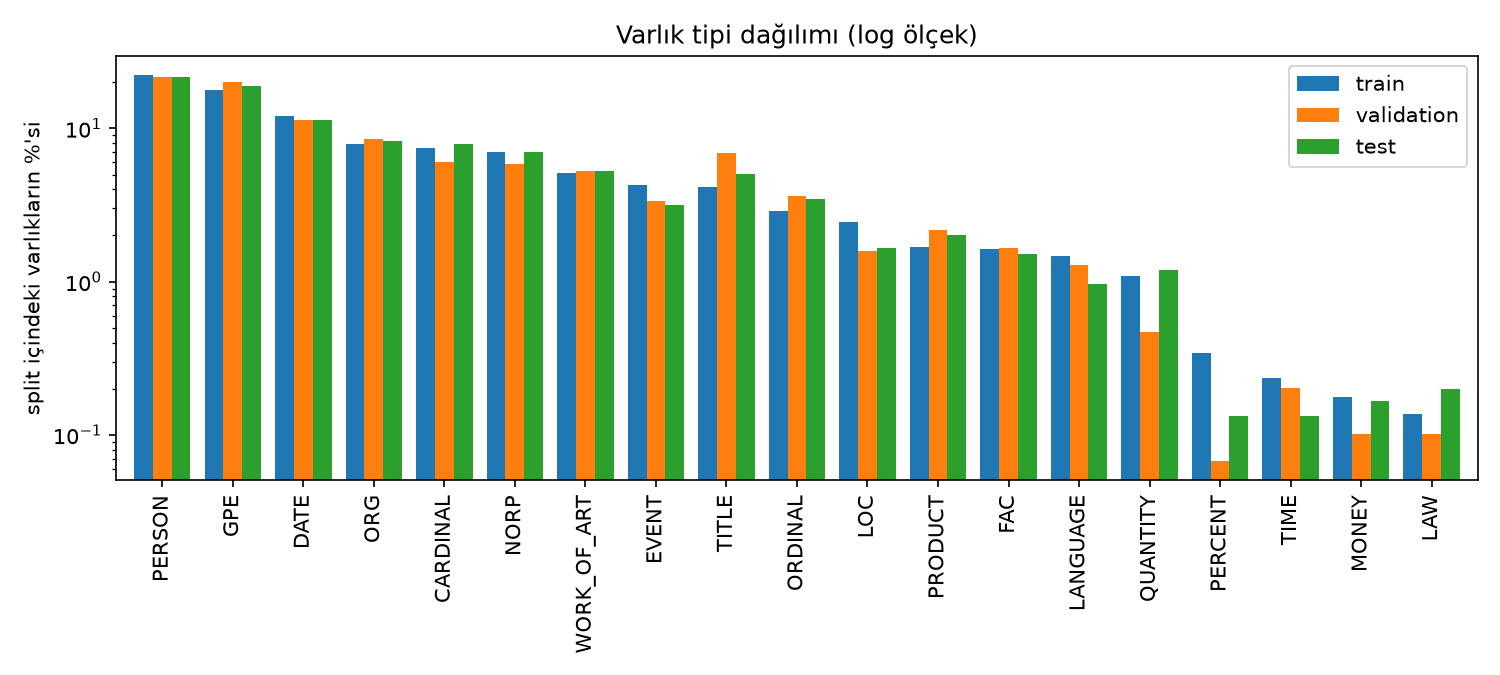
\includegraphics[width=\columnwidth]{entity_type_distribution.png}
\caption{Entity type distribution per split (log scale).}
\label{fig:types}
\end{figure}

\section{Baseline: Feature-Rich CRF}
We train a linear-chain CRF (L-BFGS, $c_1{=}c_2{=}0.05$, 150 iterations) on the given whitespace tokens.

\paragraph{Preprocessing.} We deliberately avoid lowercasing and stemming the input, because case and suffixes are signal. Instead we expose raw and normalised \emph{views} of each token as separate features.

\paragraph{Features and rationale.}
\begin{itemize}
\item \textbf{Apostrophe split} into stem and suffix (\textit{Ankara'da}$\to$\textit{ankara}+\textit{da}). The stem feature merges all inflected forms of a name, and the mere presence of a suffix is a near-deterministic cue for a proper noun.
\item \textbf{Capitalisation} features: title case, all caps, and \textit{title-and-not-sentence-initial}. Capitalisation at the beginning of a sentence carries no information.
\item \textbf{Word shape} (\textit{Xx}, \textit{dddd}, \textit{XX}) separates the numeric types (DATE, CARDINAL, PERCENT, MONEY) and acronyms.
\item \textbf{Stem affixes} (2--4 characters) capture morphological cues such as \textit{-oğlu} (PERSON), \textit{-spor} (ORG) and \textit{-ce} (LANGUAGE).
\item \textbf{A $\pm$2-word window} of the same views. Head nouns such as \textit{Üniversitesi}, \textit{Nehri} and \textit{Savaşı} decide the type of the preceding tokens.
\item \textbf{Learned label transitions} keep multi-token spans intact and suppress invalid I- tags.
\end{itemize}

\section{Deep Contextual Model: BERTurk}
We fine-tune \texttt{dbmdz/bert-base-turkish-cased} \citep{schweter2020berturk} with a linear token-classification head.

\paragraph{Why BERTurk.} It is monolingual, so its vocabulary segments Turkish morphology into fewer pieces than mBERT or XLM-R. It is cased, which preserves the capitalisation cue. Its 110M parameters fit an 8\,GB laptop GPU.

\paragraph{Tokenisation.} Words are split into WordPieces. Only the \emph{first} sub-token of each word carries the label; the rest are masked from the loss (label $-100$). Labelling every piece would over-weight long, heavily suffixed words. Predictions are read from the same first sub-token, so evaluation is word-level and directly comparable with the CRF.

\paragraph{Training regime.} 3 epochs, AdamW, learning rate $5{\times}10^{-5}$ with linear decay and 10\% warm-up, weight decay 0.01, batch size 32, fp16, maximum length 192. We select the checkpoint with the lowest validation loss and evaluate on the test set exactly once.

\section{Novel Method: Suffix-Preserving Entity Swap}
\paragraph{Hypothesis.} If the model memorises surface forms, recall on unseen entities lags far behind recall on seen ones (Table~\ref{tab:main}). Forcing the model to identify a span from its \emph{context} should close that gap.

\paragraph{Method.} Mention replacement (MR) swaps an entity for another mention of the same type. It is one of the simple augmentations studied by \citet{dai2020analysis}.

Applied naively to Turkish, MR produces ungrammatical forms such as \textit{*İzmir'a} or \textit{*Bitlis'da}. These give the model a shortcut: an ungrammatical sentence signals a swapped entity. We therefore make the replacement morphology-aware:
\begin{enumerate}
\item Build a mention bank per type from the training spans, with suffixes stripped.
\item For each training sentence that contains an entity, create one copy in which each span is replaced with probability 0.7 by a random mention of the same type.
\item If the original final token carried an apostrophe suffix, re-attach that suffix to the new stem after applying two rules. \emph{Vowel harmony}: two-way a/e and four-way ı/i/u/ü, based on the last vowel of the stem. \emph{Consonant assimilation}: d$\to$t after a voiceless consonant. Examples: \textit{Samsun'a}$\to$\textit{İzmir'e}, \textit{Ankara'da}$\to$\textit{Bitlis'te}.
\end{enumerate}
This doubles the number of entity-bearing sentences.

We did not find prior work that re-inflects Turkish suffixes during entity swaps, but our search was brief. Buffer consonants (\textit{Ankara'ya} vs.\ \textit{Paris'e}) are not modelled; we accept this residual noise.

\section{Results \& Discussion}
\begin{table}[t]
\centering\small
\begin{tabular}{lcccc}
\toprule
Model & F1 & mF1 & R$_{seen}$ & R$_{unseen}$ \\
\midrule
CRF (features) & .681 & .583 & .757 & .570 \\
BERTurk & \textbf{.810} & .720 & \textbf{.831} & \textbf{.766} \\
\quad + swap ($p{=}0.7$) & .780 & \textbf{.721} & .763 & .736 \\
\quad + swap ($p{=}0.3$) & .796 & .719 & .802 & .747 \\
\bottomrule
\end{tabular}
\caption{Test results (strict entity-level). mF1 = macro-F1; R = recall on gold entities whose surface form is seen/unseen in train (60.2\% unseen). Single seed (42).}
\label{tab:main}
\end{table}

\begin{table}[t]
\centering\small
\begin{tabular}{lrccc}
\toprule
Type & \# & CRF & BERTurk & +swap \\
\midrule
PERSON & 654 & .778 & .925 & .927 \\
GPE & 566 & .725 & .851 & .801 \\
DATE & 343 & .676 & .793 & .705 \\
ORG & 250 & .601 & .807 & .757 \\
CARDINAL & 240 & .710 & .749 & .750 \\
NORP & 212 & .706 & .773 & .800 \\
WORK\_OF\_ART & 158 & .538 & .835 & .801 \\
TITLE & 153 & .398 & .489 & .370 \\
ORDINAL & 104 & .733 & .804 & .696 \\
EVENT & 95 & .583 & .716 & .741 \\
PRODUCT & 61 & .372 & .673 & .702 \\
LOC & 50 & .473 & .660 & .563 \\
FAC & 46 & .506 & .696 & .745 \\
QUANTITY & 36 & .818 & .845 & .861 \\
LANGUAGE & 29 & .679 & .746 & .716 \\
LAW & 6 & .545 & .250 & .727 \\
\bottomrule
\end{tabular}
\caption{Per-type test F1 (MONEY, PERCENT and TIME have $\le$5 instances and are omitted).}
\label{tab:types}
\end{table}

\paragraph{CRF vs.\ BERTurk.} Contextual representations add 13 points of micro-F1 and 14 of macro-F1 (Table~\ref{tab:main}). Our fine-tuned BERTurk also exceeds the 0.76 micro-F1 reported on the dataset card \citep{altinok2023turkish}.

The gains are not uniform (Table~\ref{tab:types}). They are largest for \emph{phrasal, context-defined} types: WORK\_OF\_ART +30, PRODUCT +30, ORG +21, FAC +19. These are exactly the types where the CRF's $\pm$2 window cannot see the head noun or the sentence-level semantics. Gains are smallest for types the CRF already captures through orthography and morphology: CARDINAL +4, QUANTITY +3, NORP +7. The CRF's highest-weighted features confirm this: the suffix \textit{-lı/-li} predicts NORP, the stem ending \textit{-ca/-çe} predicts LANGUAGE, and the shape \textit{\%dd} predicts PERCENT. Turkish morphology is a cheap and strong signal.

\paragraph{Memorisation.} The CRF loses 18.7 recall points on unseen entities. BERTurk loses only 6.5, so most of its gain comes from generalising beyond the training lexicon, which matters for a corpus where 60\% of test mentions are new.

TITLE remains the weakest frequent type for both models (F1 $<$ .50). It is the one type added beyond OntoNotes, and its boundary with O (\textit{kral}, \textit{başbakan}) is inconsistently annotated. We therefore attribute a large share of these errors to label ambiguity rather than model capacity.

\paragraph{Augmentation: a negative result.} Suffix-preserving swap with $p{=}0.7$ \emph{reduced} micro-F1 by 3 points while leaving macro-F1 unchanged. It narrowed the seen/unseen gap to 2.7 points, but mainly by lowering seen recall. This agrees with \citet{dai2020analysis}: mention replacement helps in low-resource regimes but is neutral or harmful with full training data.

The per-type view shows the mechanism:
\begin{itemize}
\item \textbf{Gains on name-like, rare types}, where more surface variety is useful: LAW +.48, FAC +.05, PRODUCT +.03, EVENT +.03, NORP +.03.
\item \textbf{Losses on DATE (--.09), ORDINAL (--.11), GPE (--.05) and TITLE (--.12).} For temporal and numeric types, the span is syntactically coupled to its context (\textit{11 Temmuz 1927 tarihinde}). Swapping these spans creates implausible sentences and inconsistent span boundaries.
\item \textbf{GPE and TITLE} are among the most ambiguous types. Random swaps amplify their existing type confusion (GPE vs.\ NORP vs.\ ORG).
\end{itemize}
The actionable conclusion is that augmentation should be \emph{type-selective}: swap only name-like types (PERSON, ORG, FAC, PRODUCT, EVENT, LAW, WORK\_OF\_ART), and apply it mainly to rare types. A lower swap rate supports this reading. With $p{=}0.3$, F1 recovers to .796, DATE returns to .782 (vs.\ .793), and PRODUCT/LAW keep most of their gains. Micro-F1 decreases monotonically with swap intensity (.810 $\to$ .796 $\to$ .780), so the loss comes from the swap itself rather than from noise between runs.

\paragraph{Limitations.} All numbers come from a single seed, and differences below roughly 1 F1 point should not be over-interpreted. Rare-type F1 rests on 4--6 test instances.

\section{Production \& Future Work}
\paragraph{Production.}
\begin{itemize}
\item Export to ONNX/INT8 for CPU serving.
\item Use a word-level API that returns spans, types and confidences.
\item Monitor the predicted type distribution and the share of unseen-entity predictions to detect drift.
\item Send low-confidence spans to human review.
\end{itemize}

\paragraph{With more time and compute.}
\begin{itemize}
\item Average results over multiple seeds and report confidence intervals.
\item Add a CRF head and try larger encoders (XLM-R large, a Turkish ELECTRA or DeBERTa).
\item Gazetteer features from Wikidata.
\item Use an LLM for few-shot adjudication of low-confidence or rare-type spans, and for context-diverse data generation.
\item Find and fix noisy labels (TITLE in particular).
\end{itemize}

\bibliography{custom}

\end{document}
